\documentclass[11pt]{scrartcl}
\usepackage[utf8]{inputenc}
\usepackage{evank}


%% insert title here
\newcommand{\titlee}{Waves II}
\parindent 0 pt

\newcommand{\officialsol}[1]{See the official solutions \href{#1}{here}.}

\title{\titlee}
\author{Cambridge Physics Academy}
\date{2023-2024}


\begin{document}

\thispagestyle{empty}
\begin{center}
    
    
    \Huge \textbf{\textsf{\titlee}}

    \large \theauthor
\end{center}

\setcounter{section}{-1}
\section{Readings}
\begin{itemize}
    \item 40.3-42 of HRK
\end{itemize}
It is highly recommended to do the problems in HRK (Ch 40-42) this week for extra practice. These problems are usually plug-and-chug, but are useful in making sure you have a strong grasp of the content.


\section{Lecture review}

\begin{idea}[Mirrors and lenses]
    When finding the image of an object from a system with mirrors and lenses, tracing the paths of the following three key rays is helpful: 
    \begin{enumerate}
        \item A ray drawn parallel to the axis of the lens, which passes through the lens and through the other focus.
        \item A ray drawn directly through the center of the lens that is not deflected.
        \item A ray drawn through the nearest focus, which passes through the lens and then moves parallel to the axis.
    \end{enumerate}
    \begin{center}
        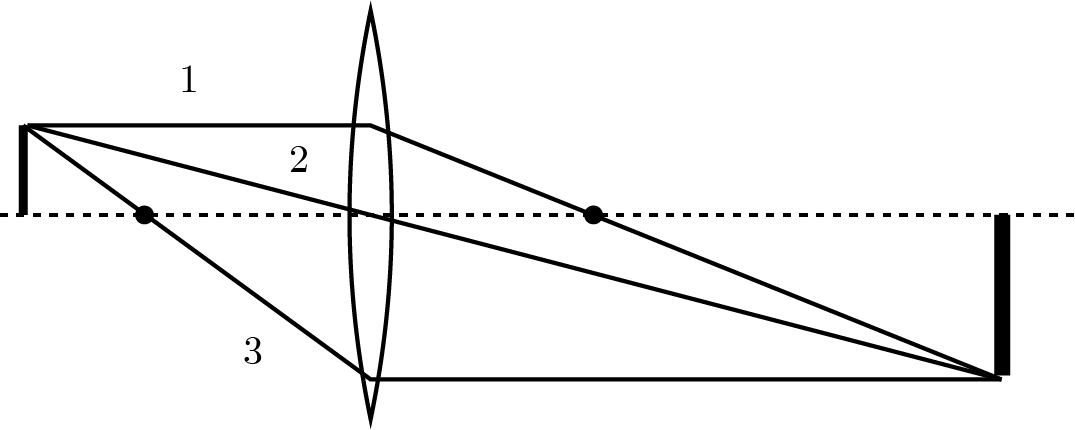
\includegraphics[scale=1]{lens2}
    \end{center}
\end{idea}

\begin{defn}[Virtual and real images]
    A real image is created when light rays from the object intersect at one point. A virtual image is created when the light rays do not actually intersect, but their extensions do. For a mirror, a real image is created when the image is on the same side of the mirror as the object, and virtual when not. For a lens, this is the opposite: real images are formed on the other side of the lens, while virtual images are created on the same side as the lens. 
\end{defn}

\begin{theorem}[Lens equation]
    For lenses (and mirrors), let the focal length be $f$, object distance $o$, and image distance $i$. The object distance is taken to be positive, and the focal distance and image distance are taken to be positive if real and negative if virtual. $$\frac1o+\frac1i=\frac1f$$
    The magnification of the image is defined to be the ratio between the final height and the initial height of the object: $$m=\frac {h'}h$$
\end{theorem}

\begin{defn}[Interference]\label{int}
    Interference occurs when two points of light of the same wavelength $\lambda$ are emitted from different locations. At places where the phase shift between the sources is 0, we observe constructive interference and at places where the phase shift is $\pi$, we observe destructive interference. For a double slit of separation $d$, the angles at which local maxima occur are found via $$\sin \theta=\frac{N\lambda}{d}$$for $N=0,1,2,\cdots$. 
\end{defn}

\begin{defn}[Diffraction]
    Within a slit of light of width $a$, we can consider multiple wave fronts. These wave fronts will interfere with one another. The local minima due to diffraction of a slit of light are found via $$\sin \theta=\frac{N\lambda}{a}$$ for $N=1,2,\cdots$. 
\end{defn}

\begin{tip}[Intensity using phasors]
    When considering the intensity of light due to interference and diffraction, first note that $I\propto E^2$. Then, since $E$ oscillates sinusoidally in an EM wave, consider $E$ to be a phasor rotating in the $xy$ axes with the $x$ component of the phasor representing the magnitude of $E$ at any given point. Then, two waves with phase shift $\phi$ will have phasors $E$ separated by that angle $\phi$, and the total magnitude of the electric can be found via phasor addition. 
\end{tip}

\section{Problem Set}

\subsection{Exercises}

\begin{prob}
    Let a model of an eye be a sphere filled with fluid of index of refraction $n$. When in air, the eye can focus parallel rays of light from infinite distances on its back surface (retina). The light rays pass through a small opening (the pupil). Find $n$. 
\end{prob}

\begin{sol}
    Observe an arbitrary light ray as shown. \begin{center}
        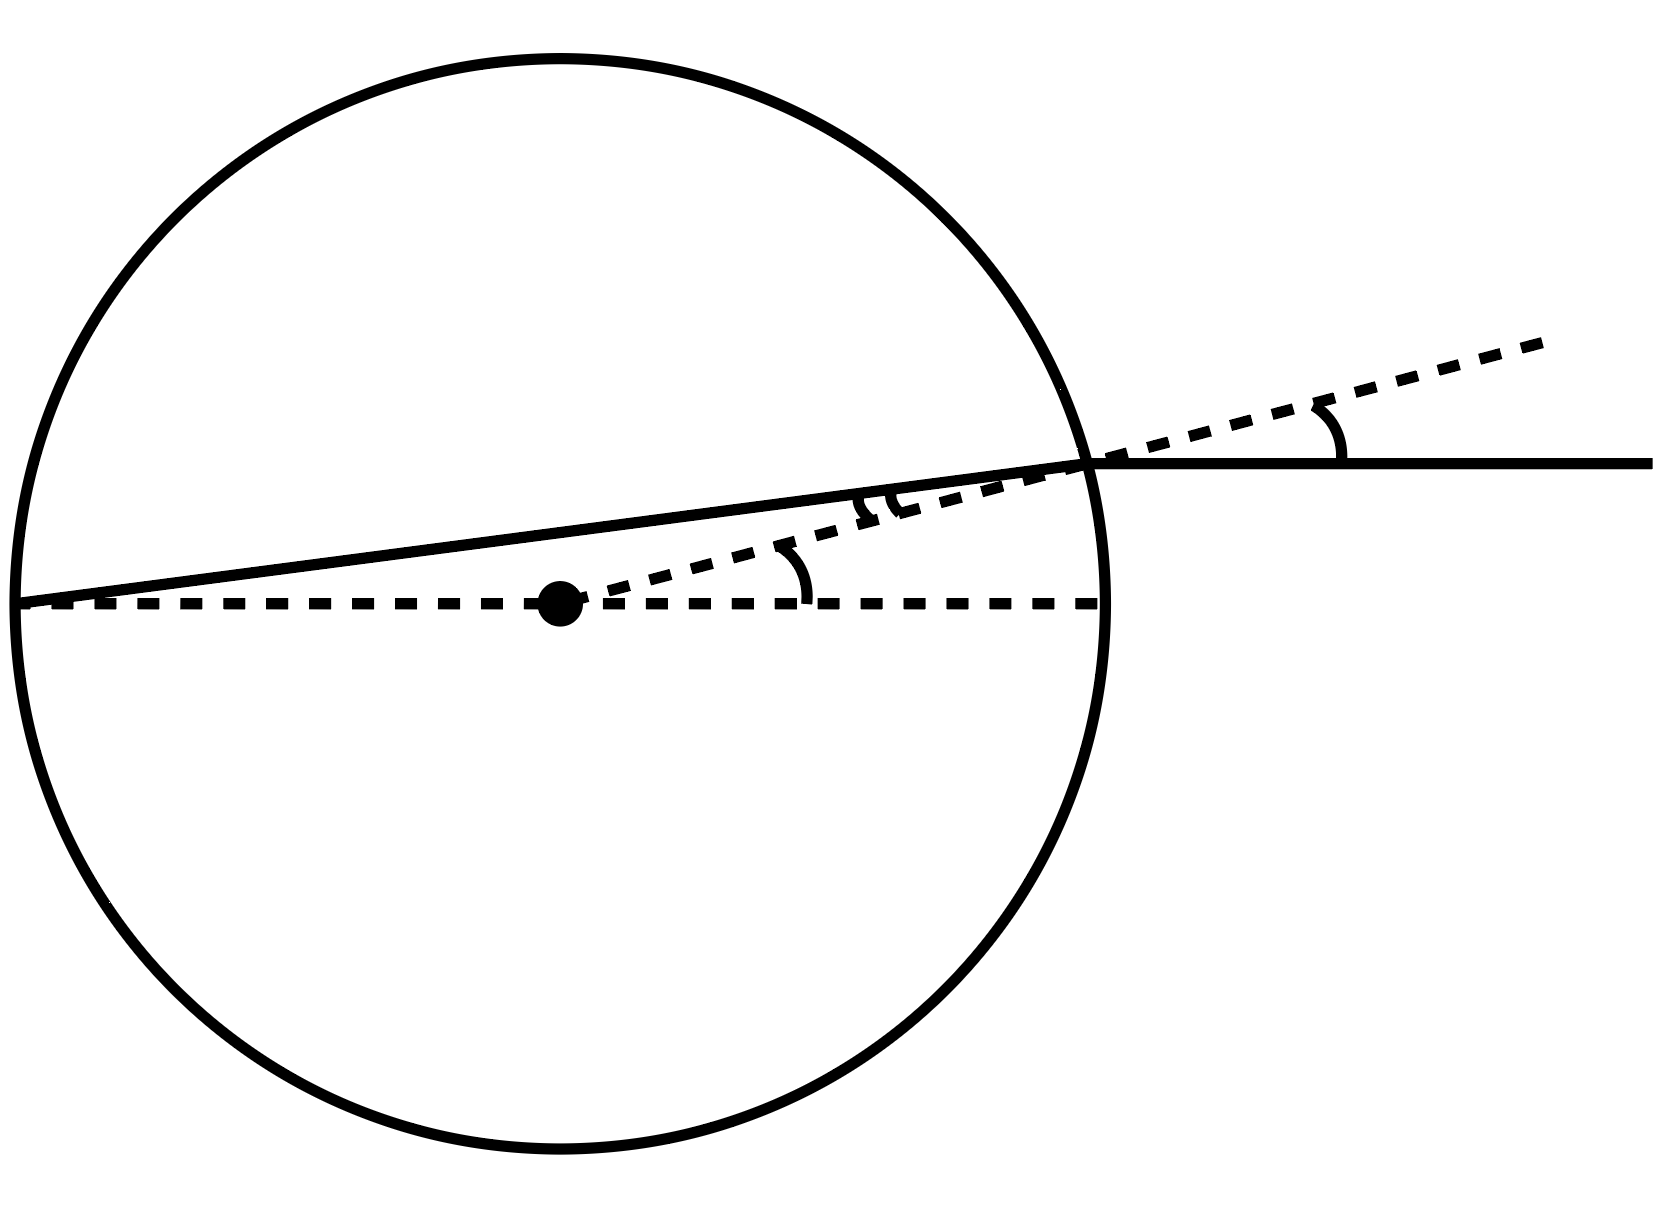
\includegraphics[scale=0.2]{eye}
    \end{center}
    By geometry, the refracted angle is half the measure of the incident angle, so by Snell's law and the small angle approximation, $\theta\cdot 1=(\theta/2)\cdot n\Rightarrow \boxed{n=2}$. 
\end{sol}

\begin{prob}
    An object is placed a distance $o=10\, \unit m$ from a convex lens with positive focal length $f=5\, \unit{m}$. Find the location and magnification of its image. 
\end{prob}

\begin{sol}
    By the lens equation, $$i=\left(\frac 1f-\frac1o\right)^{-1}=\left(\frac 1{5}-\frac1{10}\right)^{-1}=\boxed{10\, \unit m}$$The image is inverted but at the same distance away from the lens, so $\boxed{m=-1}$. 
\end{sol}

\begin{prob}
    Two identical concave mirrors of focal length $f$ are placed facing each other with their distances separated by a distance $d$ as shown. \begin{center}
        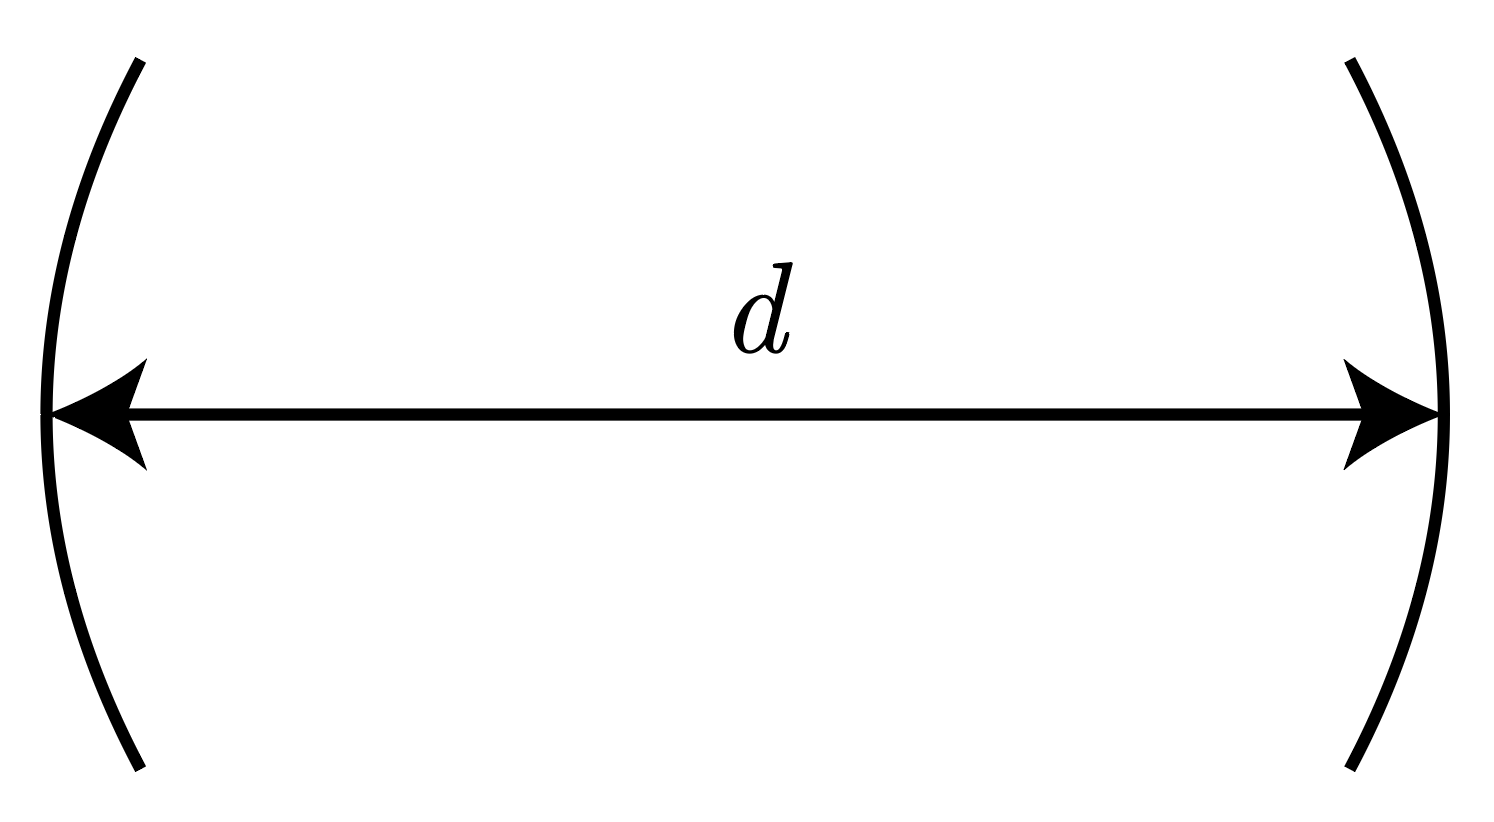
\includegraphics[scale=0.2]{miro2.png}
    \end{center}
    Depending on where an object is placed in between the mirrors, an infinite number of images can be produced. For what values of $d$ will there always be an infinite number of images, no matter where the object is placed between the mirrors?
\end{prob}

\begin{sol}
    The only case for which there would not be an infinite number of images is if an object placed exactly in between the lenses is its own image. Thus by the lens equation, $$\frac2d+\frac2d=\frac1f\Rightarrow d=4f$$ In all other cases, all objects will yield an infinite number of images, so we only require $\boxed{d\neq 4f}$. 
\end{sol}

\begin{prob}
    Given a lens of focal length $f$, find the minimum possible distance between an object and its image for nonzero object distances from the lens. 
\end{prob}

\begin{sol}
    Let the object distance be $o$. By the lens equation, $$i=\left(\frac 1f-\frac1o\right)^{-1}=\frac{of}{o-f}$$ We seek to minimize $$D=o+i=o+\frac{of}{o-f}$$Taking the derivative $d/do$ and setting to 0 yields $$1+\frac{f}{o-f}-\frac{of}{(o-f)^2}=0\Rightarrow o=2f$$ Substituting this into $D$ yields $\boxed{D=4f}$.
\end{sol}

\begin{prob}
    Newton's lens formula states that if the distances of the object and image from the first and second focal points are $x_1$ and $x_2$, respectively, then $$x_1x_2=f^2$$Derive this fact from the lens equation. 
\end{prob}

\begin{sol}
    We substitute $o=f+x_1$ and $i=f+x_2$ into the lens equation: $$\frac1{f+x_1}+\frac1{f+x_2}=\frac1f\Rightarrow f^2+x_1f+f^2+x_2f=f^2+x_1x_2+x_1f+x_2f\Rightarrow \boxed{x_1x_2=f^2}$$
\end{sol}

\begin{prob}[CP]
A wire with negligible thickness is placed a distance $o$ in front of a converging lens of unknown focal length and diameter $D$. When a screen is placed at a distance $L$ behind the lens, a smudge with an appreciable thickness $d$ is formed. Determine the possible focal lengths of the lens.
\end{prob}

\begin{sol}
    There are two possible positions of the screen that lead to a smudge of thickness $d$, as shown in the figure below. \begin{center}
        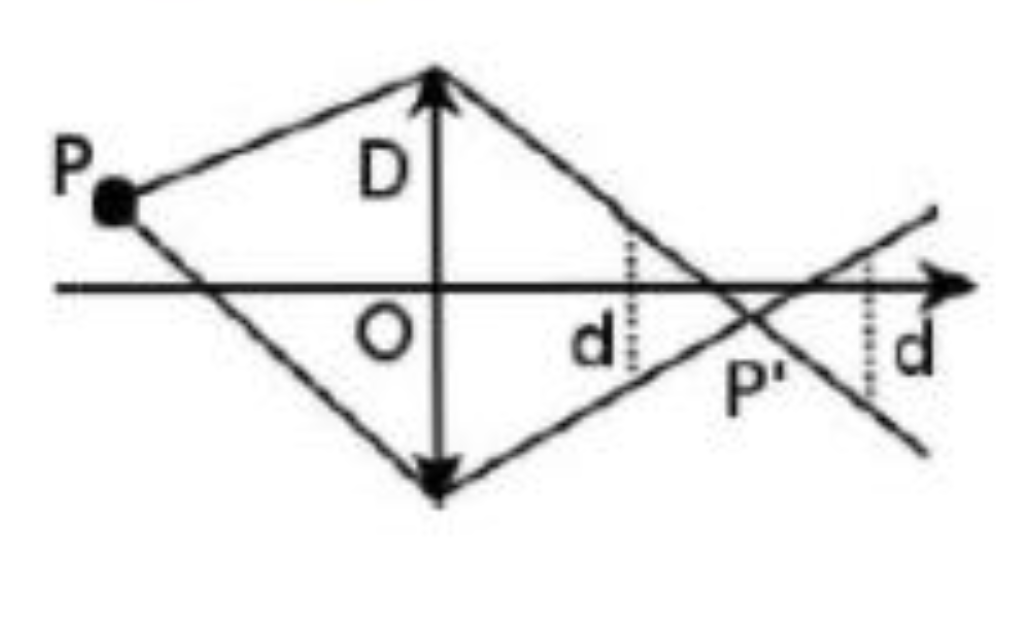
\includegraphics[scale=0.2]{cp}   
    \end{center}
    Let $i$ be the image distance, and $x$ the distance between the image and the screen. By similar triangles, $x=i(d/D)$. Thus, the two possible image distances are $i=L-x$ and $i=L+x$, and substituting $x$ yields $i=LD/(D+d)$ and $i=LD/(D-d)$. By the lens equation, we can thus find the two possible options for the focal length to be $$f=
    \boxed{\left(\frac1o+\frac{D+d}{LD}\right)^{-1}}\qquad f=\boxed{\left(\frac1o+\frac{D-d}{LD}\right)^{-1}}$$
\end{sol}

\begin{prob}[NBPhO]
A normal healthy eye is able to see an object clearly if the object is located at a distance between $25.0 \, \unit{cm}$ to infinity from the eye. A nearsighted eye sees equally well with the aid of a contact lens with an optical power of $-6.00$ dioptres. (A diopter is equal to 1 $\unit{m^{-1}}$, and the optical power is the reciprocal of the focal length). 
\begin{anum}
    \item What is the clear‐vision range for the nearsighted eye without the contact lens?
    \item  If a person uses glasses instead of contact lenses and the lens in the glasses is 2.00 cm from the eye, what is the adequate optical power of the lens to aid the nearsighted eye to see normally?
\end{anum}
\end{prob}

\begin{sol}
    See solutions \href{https://nbpho.ee/wp-content/uploads/2022/NBPhO_2022_solutions.pdf}{here} (Problem 6, parts i and ii).
\end{sol}

\begin{prob}
    Consider a two-slit experiment with slit separation $d$ and light of wavelength $\lambda$. Somehow, the light through the top slit is a phase angle $\phi$ ahead of the bottom slit, where $0\leq \phi \leq 2\pi$. The screen is a distance $L$ away from the slits. 
    \begin{anum}
        \item Find the location $y$ of the $N$th local maximum (counting up from the center) if $\phi=\pi$. Assume $y\ll L$. 
        \item Find the location $y$ of the $N$th local maximum if $\phi=\pi/2$. Assume $y\ll L$.
        \item Now, let $\phi$ vary linearly as a function of time: $\phi=\alpha t$. Find the velocity of the wave pattern on the screen for positions $y\ll L$.
        \item Find the answer to part (c) as a function of $y$ if we no longer assume $y\ll L$. 
    \end{anum}
\end{prob}

\begin{sol}
    \begin{anum}
        \item If $\phi=\pi$, then all the maxima become minima, and all the minima become maxima. In other words, the pattern is shifted a distance $\lambda L/2d$ upwards, by Definition \ref{int}. Thus the $N$th local maximum is found at location $$y_N=\frac{(N-1+\frac12)\lambda L}{d}=\boxed{\frac{(N-\frac12)\lambda L}{d}}$$
        \item The condition for the first maximum is that we need to overcome a quarter wavelength, so $\theta d=\lambda/4$. Thus everything is shifted by a factor $1/4$ instead of $1/2$ as in part (a): 
        $$y_N=\frac{(N-1+\frac14)\lambda L}{d}=\boxed{\frac{(N-\frac34)\lambda L}{d}}$$
        \item The frequency is $\alpha/2\pi$, and the wavelength of the interference pattern (distance between adjacent maxima) is $\lambda L/d$. Thus $$v=\boxed{\frac{\alpha \lambda L}{2\pi d}}$$
        \item Since the angular separation between two adjacent maxima is small,  we can find it via taking a derivative $$\sin\theta=\frac{N\lambda}{d}\Rightarrow \cos\theta \, d\theta=\frac{\lambda}{d}$$Now, note that from geometry, $$dy=\frac{L\, d\theta}{\cos^2\theta}=\frac{\lambda L}{d\cos^3\theta}$$This is the precise wavelength of the interference pattern. As a function of $y$, we have $\cos^3\theta=L^3/(L^2+y^2)^{3/2}$ so that $$v=\frac{\alpha\lambda L}{2\pi d}\frac{\sqrt{(L^2+y^2)^3}}{L^3}=\boxed{\frac{\alpha\lambda \sqrt{(L^2+y^2)^3}}{2\pi L^2d}}$$
    \end{anum}
\end{sol}

\begin{prob}[HRK]
The figure below shows a plano-convex lens of radius of curvature $R$ resting on a planar glass plate illuminated directly from above by parallel light rays of wavelength $\lambda$. 
\begin{center}
    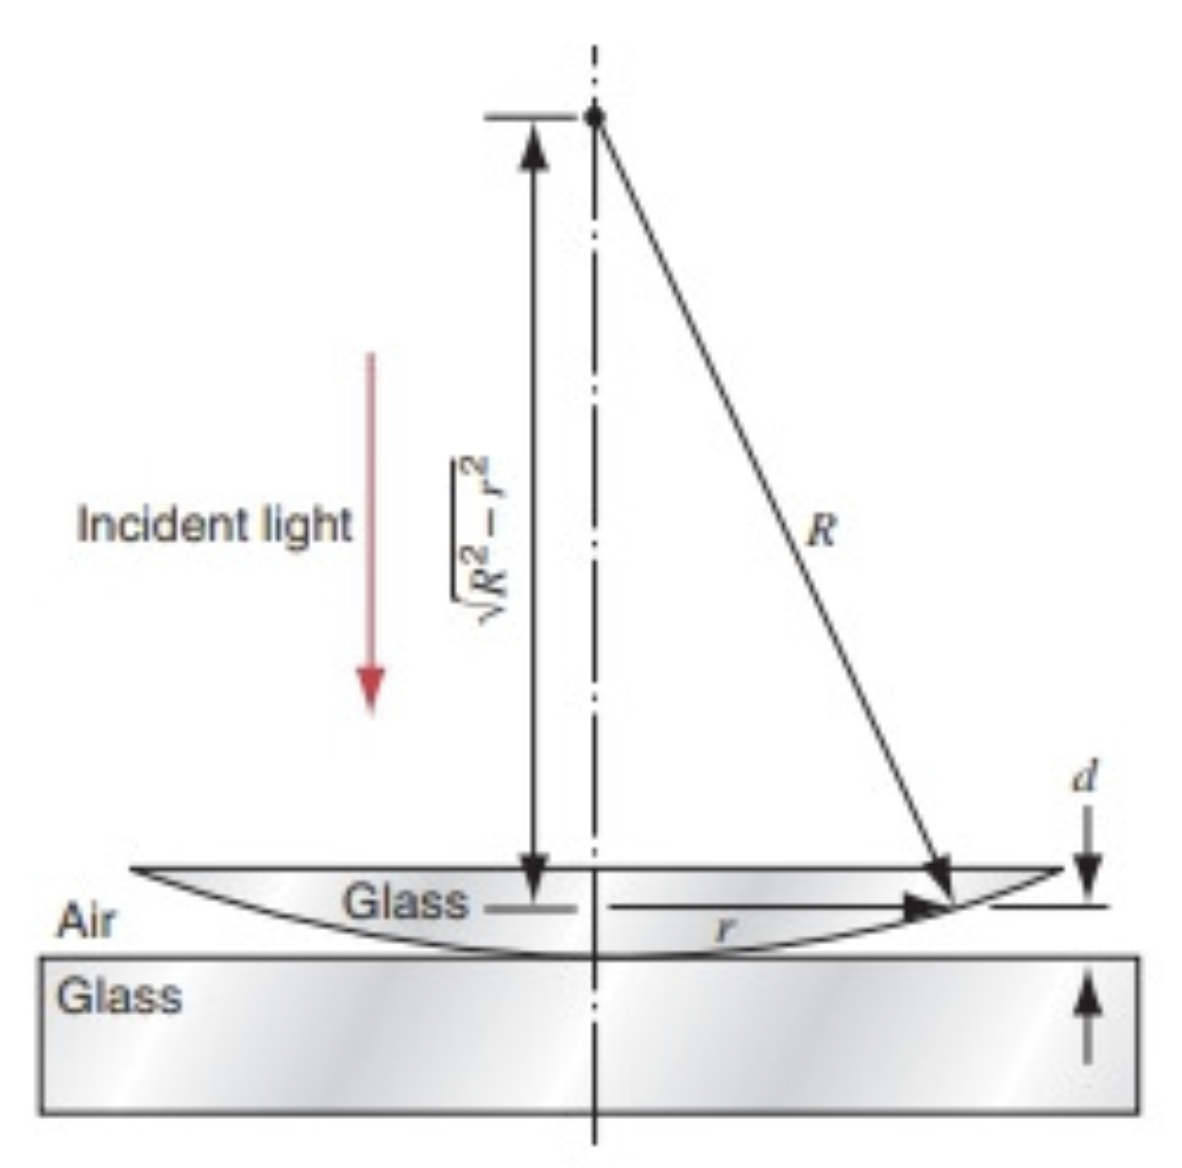
\includegraphics[scale=0.25]{hrk1}
\end{center}
Circular interference rings called Newton's rings appear when the apparatus is viewed from above. \begin{anum}
    \item Find the radii of the circular interference maxima in terms of $m=1,2,\cdots$. 
    \item Find the area between adjacent rings (maxima) for $m\gg 1$ and show that it is independent of $m$.
\end{anum}
\end{prob}

\begin{sol}
    \begin{anum}
        \item As in the figure, a light ray bouncing off of the bottom surface of the lens receives no phase shift, while a light ray that reflects off the glass plane needs to travel an extra $2d$ and experiences a phase shift of half a wavelength. Thus the condition for a maximum is $$2d=\left(m-\frac12\right)\lambda$$Note that $$d=R-\sqrt{R^2-r^2}\approx R-\left(R-\frac{r^2}{2R}\right)\approx \frac{r^2}{2R}$$Plugging this value in for $d$ and solving for $r$ yields $$r=\boxed{\sqrt{\left(m-\frac12\right)\lambda R}}$$
        \item The area between rings $r_m$ and $r_{m+1}$ is $$A=\pi (r_{m+1}^2-r_m^2)=\boxed{\pi\lambda R}$$which is independent of $m$ as desired. 
    \end{anum}
\end{sol}

\begin{prob}[HRK]
    A ship approaching harbor is transmitting at a wavelength $\lambda$ from its antenna located at a height $h$ above sea level. The receiving station antenna is a height $H$ above sea level. What is the horizontal distance $D$ between ship and receiving tower when radio contact is momentarily lost for the first time? Assume the ocean is perfectly flat and reflects waves according to the law of reflection. 
    \begin{center}
    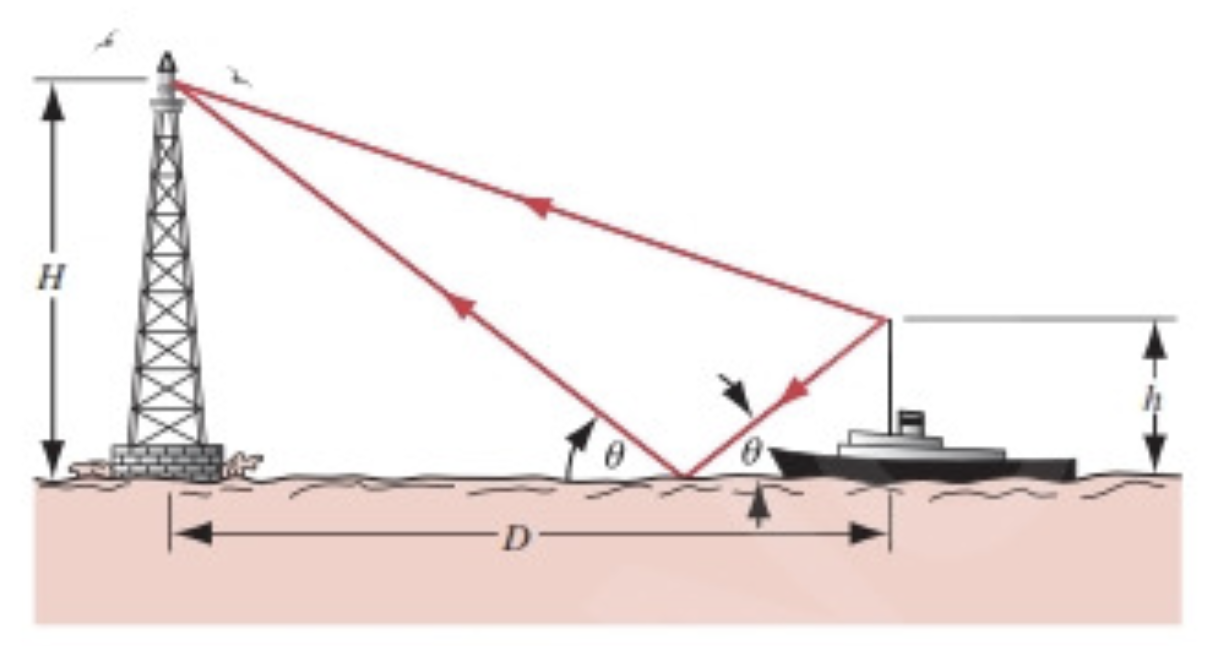
\includegraphics[scale=0.3]{hrk2}
\end{center}
\end{prob}

\begin{sol}
    Pretend the ship is a two point source emitter, one $h$ above the water, and one $h$ below the water (we can do this because $\lambda$ is very small, so $\theta$ is very small). The one below the water is out of phase by half a wavelength. Then $d\sin\theta=\lambda$, where $d = 2h$, gives the angle for theta for the first minimum. Note also that $\theta\approx H/D,$ so $$\frac{2hH}{D}=\lambda\Rightarrow D=\boxed{\frac{2hH}{\lambda}}$$
\end{sol}

\begin{prob}
    For circular apertures (instead of slits), the first diffraction minimum occurs at $$\sin\theta=\frac{1.22\lambda}{d}$$ where $d$ is the diameter of the aperture. Let there be two stars (point sources) emitting light of wavelength $\lambda$ at a total distance $r$ from an observer. Let the diameter of an eye's pupil be $d$. Rayleigh's criterion for resolving images says that you can identify the two point sources (resolve them) if the location of one source is at least as far away as the first diffraction minimum of the other. What is the minimum distance $\ell$ between the stars so that you can resolve them?
\end{prob}

\begin{sol}
    The angular separation between the stars must be at least $\theta$, so we have $$\frac{\ell}{r}=\frac{1.22\lambda}{d}\Rightarrow \ell=\boxed{\frac{1.22\lambda r}{d}}$$
\end{sol}

\begin{prob}
    Light of wavelength $\lambda$ falls on a single slit of width $a$. What is the ratio of the intensity of light at the first (non-central) maximum to the central maximum?
\end{prob}

\begin{sol}
    We derived during lecture that as a function of $\alpha=\pi \theta a/\lambda$, the intensity ratio follows $$I=I_0\left(\frac{\sin\alpha}{\alpha}\right)^2$$The first maximum is approximately in between the first two minima, so it is placed at an angle $\theta=3\lambda/2a$. Plugging this in, the ratio is $$\frac{I}{I_0}=\left(\frac{\sin 3\pi/2}{3\pi/2}\right)^2=\boxed{\frac{4}{9\pi^2}}$$
\end{sol}

\subsection{Challenge Problems}

\begin{prob}[EstPhO]
By taking measurements from the photo below, determine the diameter of the camera lens used for this photo. You can assume that images created by this camera lens are identical to ones created by ideal thin lens of matching focal length and diameter. Hint: Notice the blurry circles in the image. 
\begin{center}
    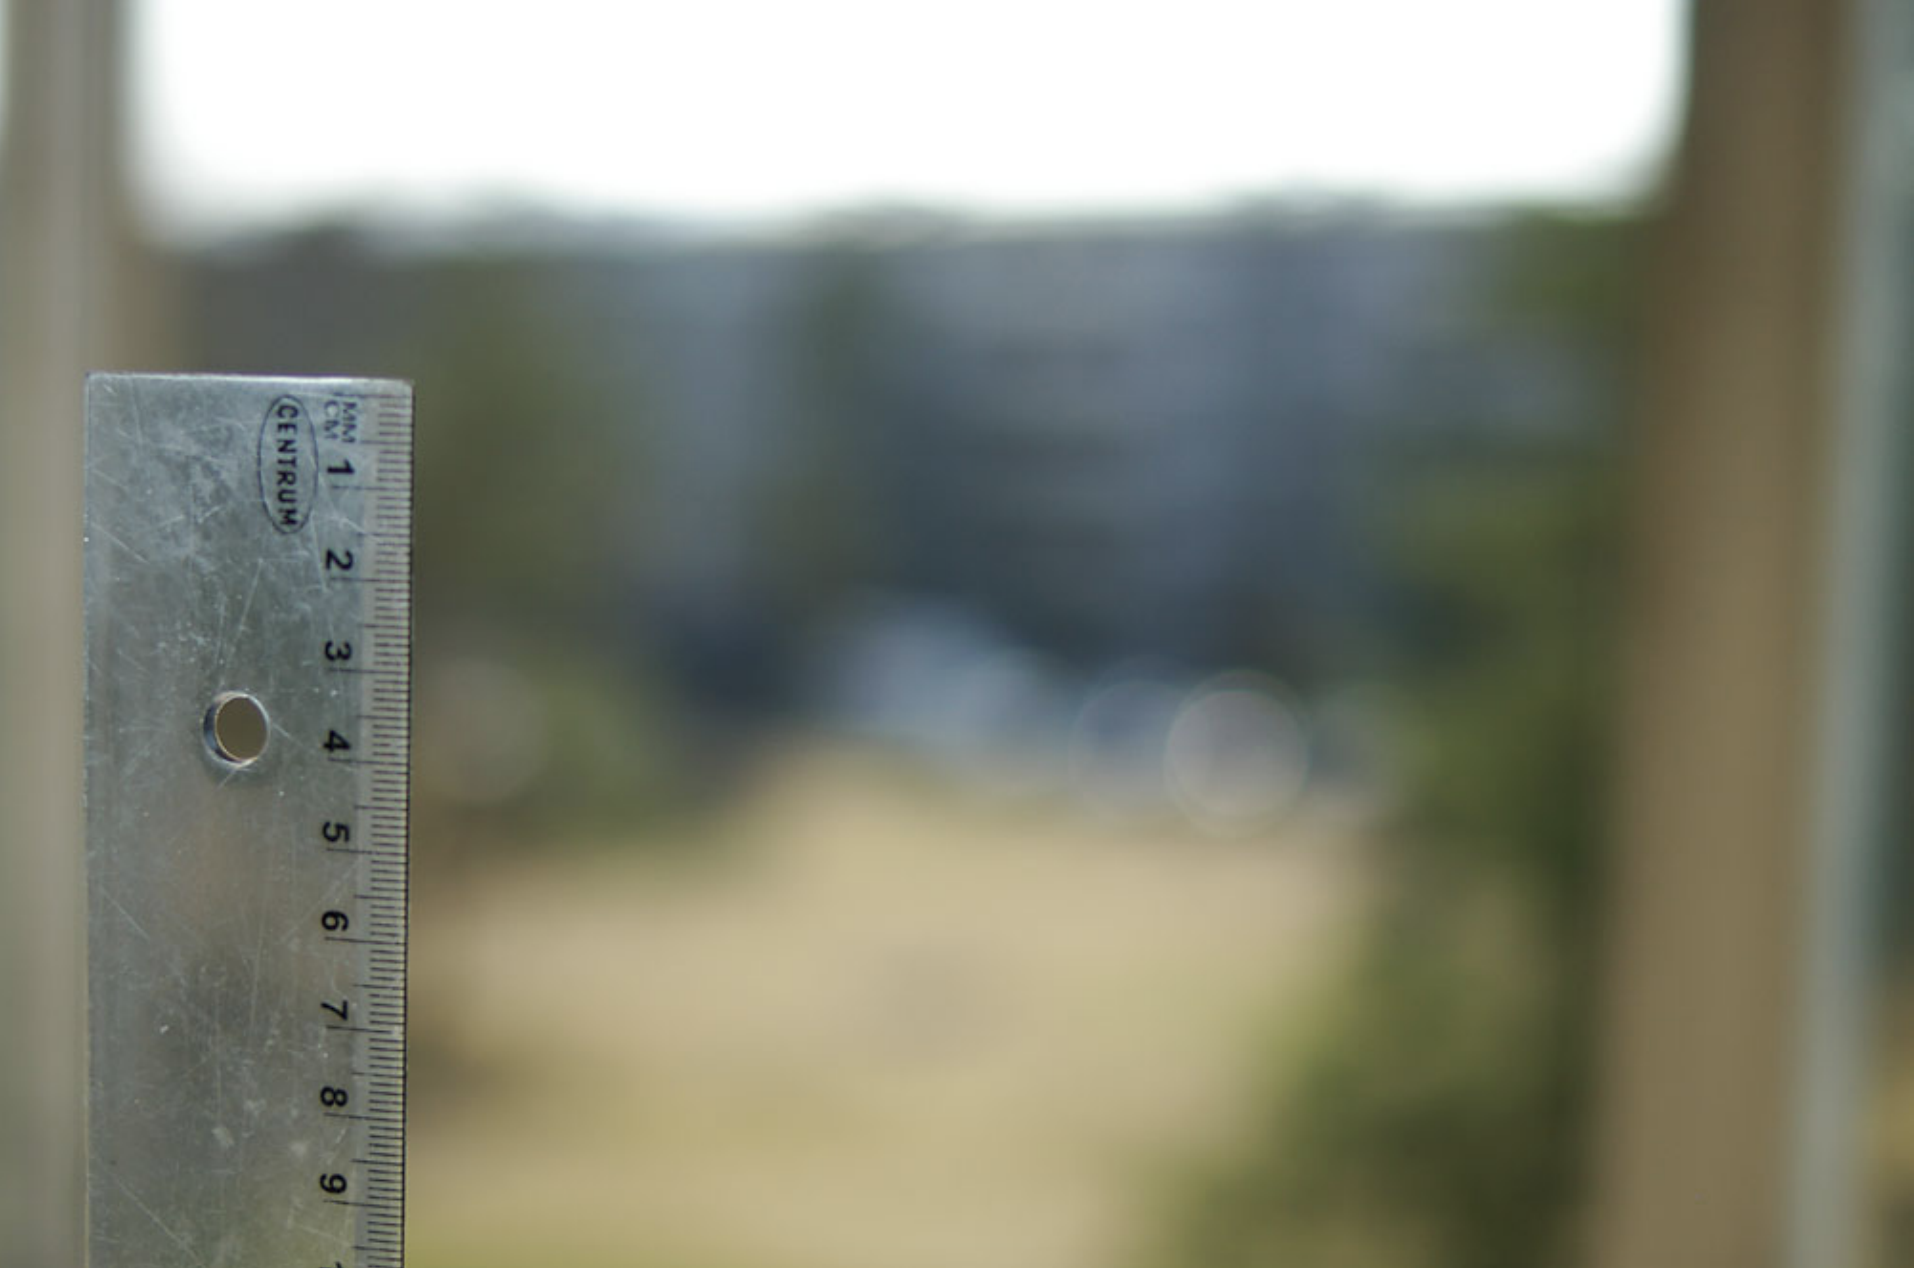
\includegraphics[scale=0.25]{photography.png}
\end{center}
\end{prob}

\begin{sol}
    See solutions \href{https://www.ioc.ee/~kalda/ipho/es/E_S_2006_sol.pdf}{here} (Problem 2).
\end{sol}

\begin{prob}[NBPhO]
    Here is a photo of a dragon under water. The length of the dragon is $l = 8\, \unit{cm}$ and its height is $h = 3\, \unit{cm}$. The diameter of the bottom of the bowl is $d = 10\, \unit{cm}$ and the angle between the table and the side of the bowl is $\alpha= 60^\circ$. The refractive index of water is $n = 1.33$. The photo has been taken so that the camera was pointing directly along the water surface. In the following questions the angle between the horizon when looking at some point on the image of the dragon is defined as the angle between the horizontal water surface (or any other horizontal surface) and the straight line from the eye to that point on the image.
    \begin{center}
        
\includegraphics[scale=0.23]{nbpho}
    \end{center}
    \begin{anum}
        \item What is the largest angle below the horizon from which the reflection of the dragon from the water surface can be seen?
        \item What is the highest angle above the horizon from which this reflection can be seen?
    \end{anum}
\end{prob}

\begin{sol}
    See solution \href{https://www.ioc.ee/~kalda/ipho/es/NBPhO17_sol.pdf}{here} (Problem 1).
\end{sol}

\subsection{USAPhO Practice}

\begin{prob}[USAPhO 2020 B2]
    Consider a square room with side length $L$. The bottom wall of the room is a perfect mirror. A perfect monochromatic point source with wavelength $\lambda$ is placed a distance $d$ above the center of the mirror, where $\lambda \ll d\ll L$.
    \begin{center}  
\includegraphics[scale=0.35]{usapho1}\end{center}
    \begin{anum}
        \item On the right wall, an interference pattern emerges. What is the distance $y$ between the bottom corner and the closest bright fringe above it? Hint: you may assume $\lambda \ll y \ll L$ as well.
        \item You plan on running an experiment to determine $\lambda$ in a room with $L = 40 \, \unit m$, and you know that $\lambda$ is between 550 and 750 nm. You will measure $d$ and $y_{10}$ (the distance of the tenth fringe from the corner) with the same ruler (with markings of 1 mm). At what $d$ should you place the point source to minimize your error in your $\lambda$ measurement? Roughly what is that minimum error?
        \item Now suppose we place a transparent hemispherical shell of thickness $s$ and index of refraction $n$ over the source such that all light from the source that directly strikes the right wall passes through the shell, and all light from the source that strikes the mirror first does not pass through the shell. \begin{center}
            
\includegraphics[scale=0.32]{usapho2}
        \end{center} At what $y$ is the fringe closest to the bottom-most corner now? (You may find it convenient to use $\lfloor x\rfloor$, the largest integer below $x$.) What is the spacing between the fringes now? Ignore any reflections or diffraction from the hemispherical shell.
        \item Now, suppose the hemispherical shell is removed, and we instead observe the interference pattern on the top wall. To the nearest integer, what is the total number of fringes that appear on the top wall? You may assume that $d\ll L$.
    \end{anum}
\end{prob}

\begin{sol}
    See solutions \href{https://aapt.org/Common/upload/2020_USAPhO_solutions.pdf}{here}. 
\end{sol}

\begin{prob}
    On a sunny day, a child with a magnifying glass wants to burn a hole through a piece of paper. Here we will examine how this may be done. Let the temperature of the sun be $T_\odot$, the radius of the sun $R_\odot$, and the distance from the sun to the Earth $r$. The magnifying glass is a convex lens with focal length $f$ and diameter $d$. The Stefan-Boltzmann constant is $\sigma.$
    \begin{anum}
        \item What is the radius of the image of the sun after passing through the magnifying glass? 
        \item Suppose some object were placed in the position of the image of the sun. What is the heat transfer per unit time to the object?
        \item Now, let this object be a thin piece of paper with emissivity $\epsilon$ and absorptivity $\alpha >\epsilon$, oriented parallel to the plane of the magnifying glass. What is the temperature of the paper?
        \item Paper burns at a temperature $T_b<T_\odot$. What is the upper bound on the ratio $\alpha/\epsilon$ to avoid burning?
        \item If we assume the paper does not burn, find the equilibrium temperature of the paper if $T_\odot=5700 \, \unit K$, $d=5\, \unit {cm}$ and $f=10\, \unit{cm}$. Compare your value to $T_b=500\, \unit K$.
    \end{anum}
\end{prob}

\begin{sol}
    \begin{anum}
        \item By the lens equation, the image position is $$i=\left(\frac 1f-\frac1r\right)^{-1}=\frac{rf}{r-f}$$ so by similar triangles the radius of the sun's image is $${R_\odot}'=R_\odot \frac{i}{r}=R_\odot \frac{f}{r-f}\approx \boxed{R_\odot\frac fr}$$
        \item The total radiation from the sun is $4\pi \sigma R_\odot^2T_\odot^4$, and a fraction $(\pi d^2/4)/(4\pi r^2)$ reaches the magnifying glass. Thus the total power arriving at the object is $$P=4\pi \sigma R_\odot^2T_\odot^4\frac{d^2}{16r^2}=\boxed{\pi \sigma R_\odot^2T_\odot^4\frac{d^2}{4r^2}}$$
        \item The paper will have total surface area $2\pi R_\odot'^2$ (considering both sides of the paper). Then, we have $$\epsilon P=\alpha(2\pi R_\odot'^2)\sigma T^4\Rightarrow T=\boxed{T_\odot 
        \left(\frac{\epsilon d^2}{8\alpha f^2}\right)^{1/4}}$$
        \item Setting $T=T_b$ and solving for $\alpha/\epsilon$ yields $$\frac\alpha\epsilon=\boxed{\frac{d^2T_\odot^4}{8f^2T_b^4}}$$
        \item By Kirchoff's Law of Radiation, in thermal equilibrium we can take $\epsilon=\alpha$ so we have $$T=(5700 \, \unit K)\left(\frac{(5\, \unit {cm})^2}{8(10\, \unit {cm})^2}\right)^{1/4}=\boxed{2400\, \unit K}$$This is way larger than $T_b$, so the paper will definitely burn!!
    \end{anum}
\end{sol}


\end{document}